\chapter{Implementation of Use Case Application}

%- Appendix: Mer detaljert beskrivelse av din implementasjon som et appendix (antall kodelinjer, biblioteker brukt, struktur, etc., alle mulige skjermbilder)

Following are a more detailed description of the iPhone application, developed as part of this project.


\section{Overview}
The implementation of the use case application, was conducted throughout the spring semester 2013, and was a continuously working progress. All implementation was done by the student itself, but the news delivery system that worked as the back-end was provided by the Department of Computer and Information Science, NTNU and other collaborators. A video demonstration of the application can be found at \url{http://youtu.be/3HgvnlqZ67A}. No code samples will be provided in this appendix, but the whole project is submitted as an external file with the project delivery, and if the code itself is of interest, it is all included in the submitted file.

\subsection{Technical Specifications}
\begin{tabular}{p {30mm} l }

\textbf{IDE}		&	Xcode Version 4.6.2 (4H1003)				\\

\textbf{Devices}	&	iPhone (3GS, 4, 4S, 5), iPod touch (3rd, 4th, 5th generation) \\

\textbf{OS}			&	Requires iOS 6.0 and above \\

\textbf{Programming language}	&	Objective C \\

\textbf{Code lines}	&	4500 \\

\textbf{Design pattern} 	& 	Model-View-Controller \\

\end{tabular}

% \section{Structure}
% The application is developed in a Model-View-Controller fashion and every view in the application has a model and a controller connected with it. 


\section{External Libraries}
Following are a quick description of the external libraries that the application makes use of.

\subsubsection{SVPullToRefresh}
\url{https://github.com/samvermette/SVPullToRefresh}\\

SVPullToRefresh is an extension control to UIScrollView that makes it possible to swipe and release to update the data in the UIScrollView.

It is used in the front page, figure \ref{usecase_frontpage}, to be able to refresh the top stories in from the front page.


\subsubsection{SVProgressHud}
\url{https://github.com/samvermette/SVProgressHUD}\\

SVProgressHud is an information control to help display messages to the user, be it progress, a success or failure message or loading. It is a singleton instance, which makes easy to use from wherever by calling its class methods.

The control is used a lot throughout the application, for instance when loading news, updating news, loading or saving the user profile, or when an article is saved.


\subsubsection{SKBounceAnimation}
\url{https://github.com/khanlou/SKBounceAnimation}\\

SKBounceAnimation is a library that makes it easier to implement a bounce effect when animating views.

This effect is used whenever a new view is loaded in the application.


\subsubsection{TestFlight SDK 1.2.4}
\url{https://testflightapp.com/sdk/}\\

The TestFlight SDK provides usage statistics, remote crash reports and logging, as well as making it possible to install the application for test purposes on remote devices.

This library is used to log checkpoints when a user is using the application, check remote crash reports and testing the application on remote devices.


\subsubsection{CMPopTipView}
\url{https://github.com/chrismiles/CMPopTipView}\\

The CMPopTipView offers an easy way to implement pop-up views that point to certain views associated with some text.

This control is used on the first launch of the application to explain how it is used, and what features that are available.


\subsubsection{KLExpandingSelect}
\url{https://github.com/KieranLafferty/KLExpandingSelect}\\

KLExpandingSelect offers a neat control to share and star content. It does not include the sharing itself, but the UI to trigger the different events.

This control is used to offer the user an opportunity to share news articles in an easy way to Twitter, Facebook and mail, as well as saving articles for accessing later (see figure \ref{usecase_share}).


\section{Screenshots}
Following are screenshots from all the screens in the application.

\begin{figure}[!htbp]
\centering
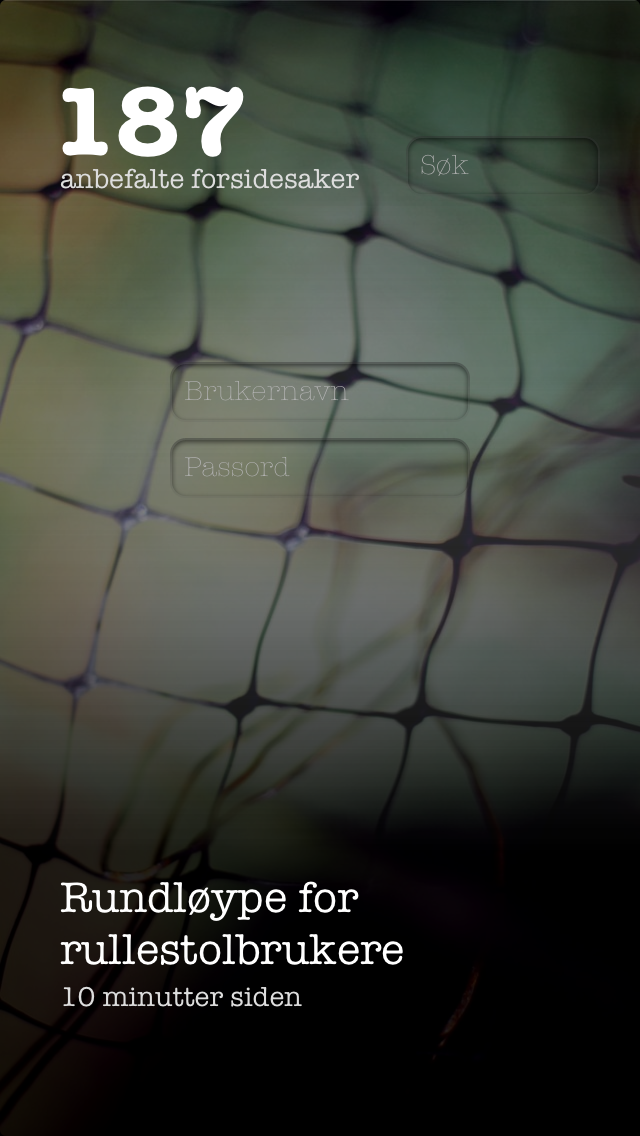
\includegraphics[width=49mm]{GFX/usecase/front.png}
\caption{Screenshot of the use case application showing the front page screen.}
\label{usecase_frontpage}
\end{figure}

\begin{figure}[!htbp]
\centering
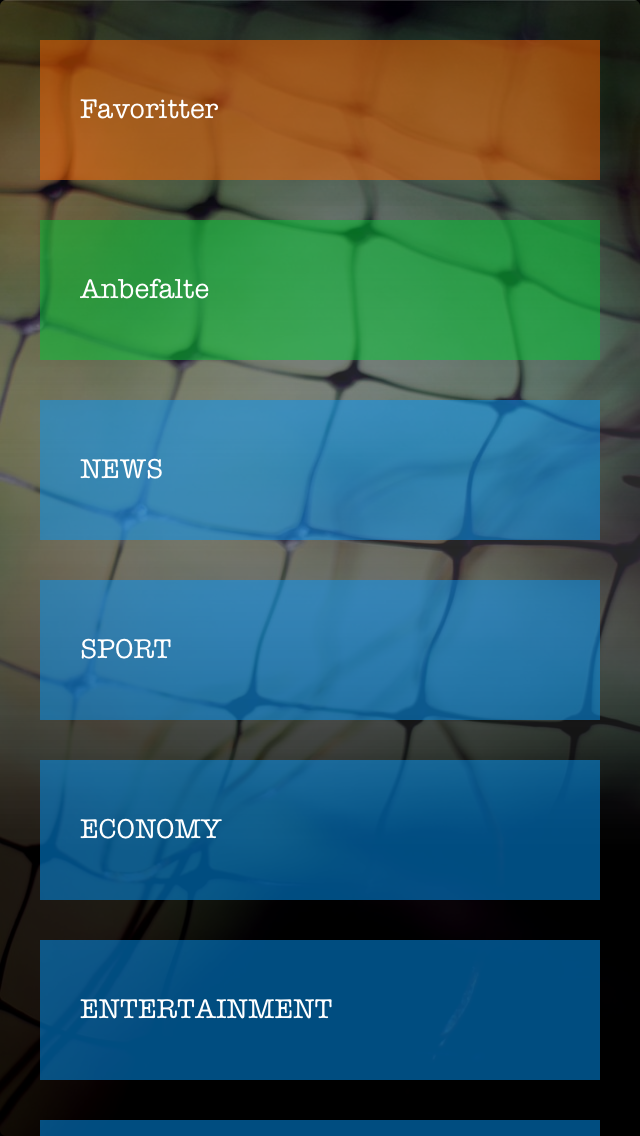
\includegraphics[width=49mm]{GFX/usecase/category.png}
\caption{Screenshot of the use case application showing the category selection screen.}
\label{usecase_category}
\end{figure}

\begin{figure}[!htbp]
\centering
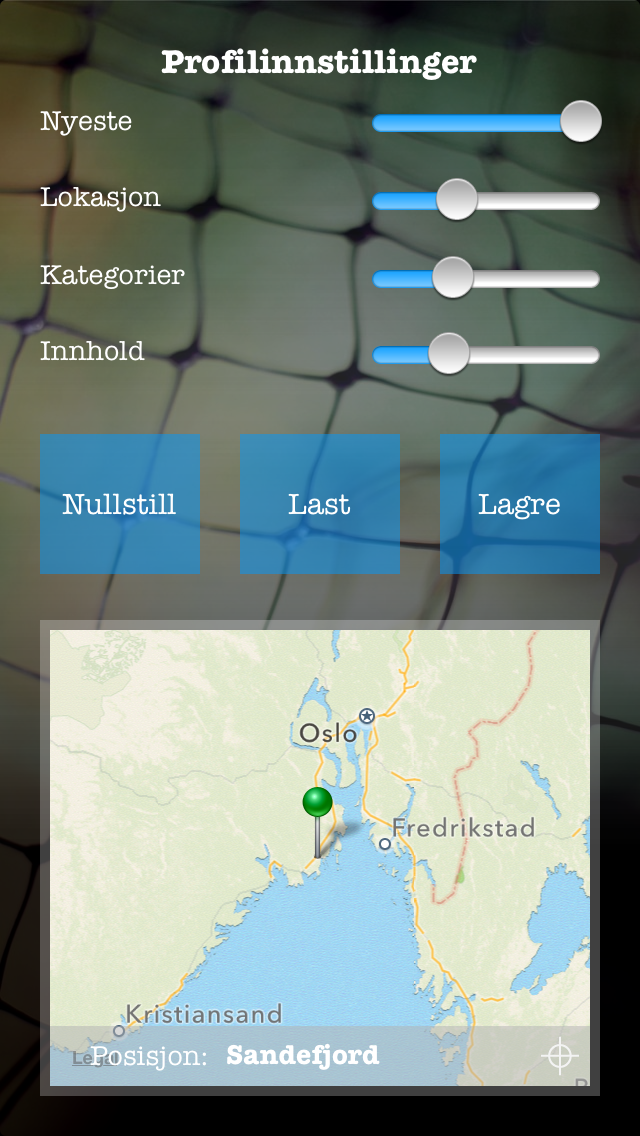
\includegraphics[width=49mm]{GFX/usecase/settings.png}
\caption{Screenshot of the use case application showing the settings screen.}
\label{usecase_settings}
\end{figure}

\begin{figure}[!htbp]
\centering
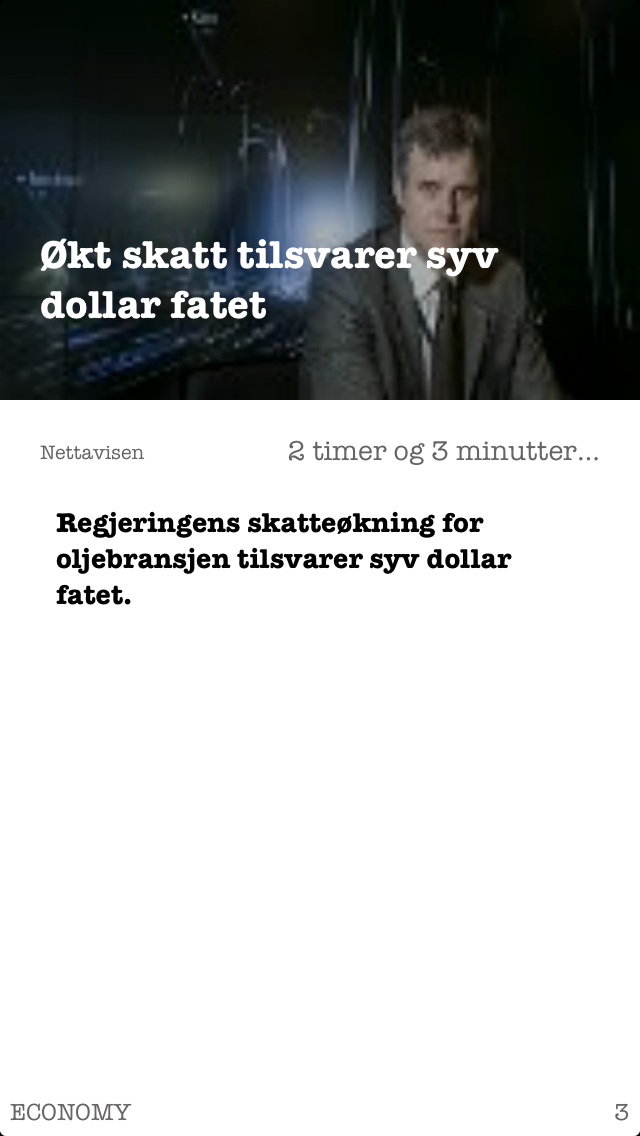
\includegraphics[width=49mm]{GFX/usecase/rssEconomy.png}
\caption{Screenshot of the use case application showing the RSS perspective.}
\label{usecase_rss}
\end{figure}

\begin{figure}[!htbp]
\centering
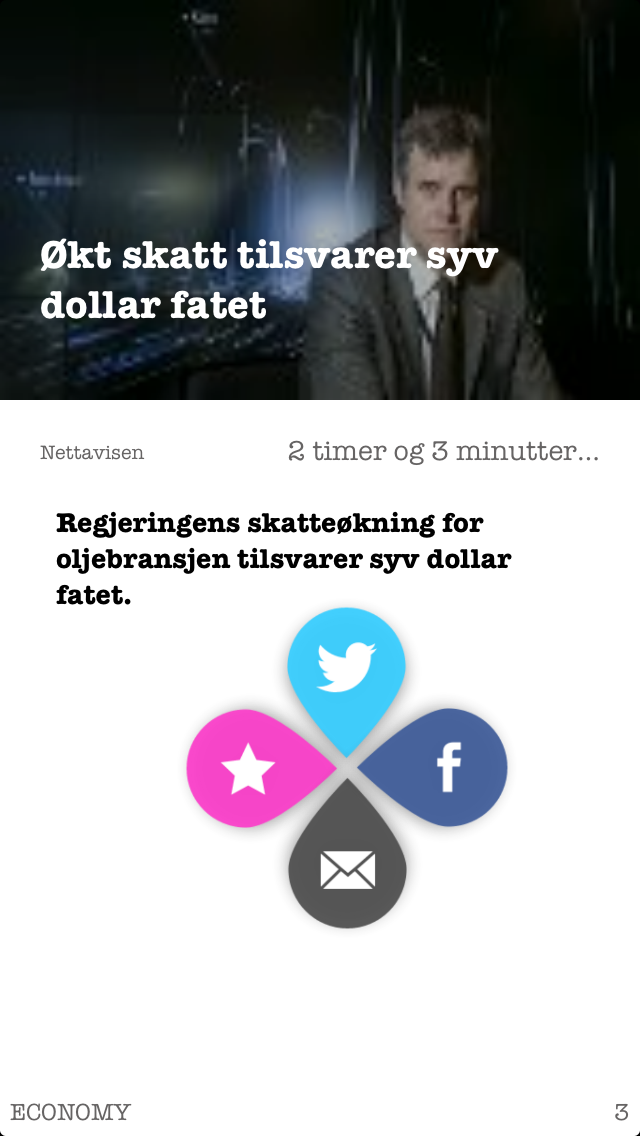
\includegraphics[width=49mm]{GFX/usecase/rssShare.png}
\caption{Screenshot of the use case application showing the RSS perspective after triggering the share/save control.}
\label{usecase_share}
\end{figure}

\begin{figure}[!htbp]
\centering
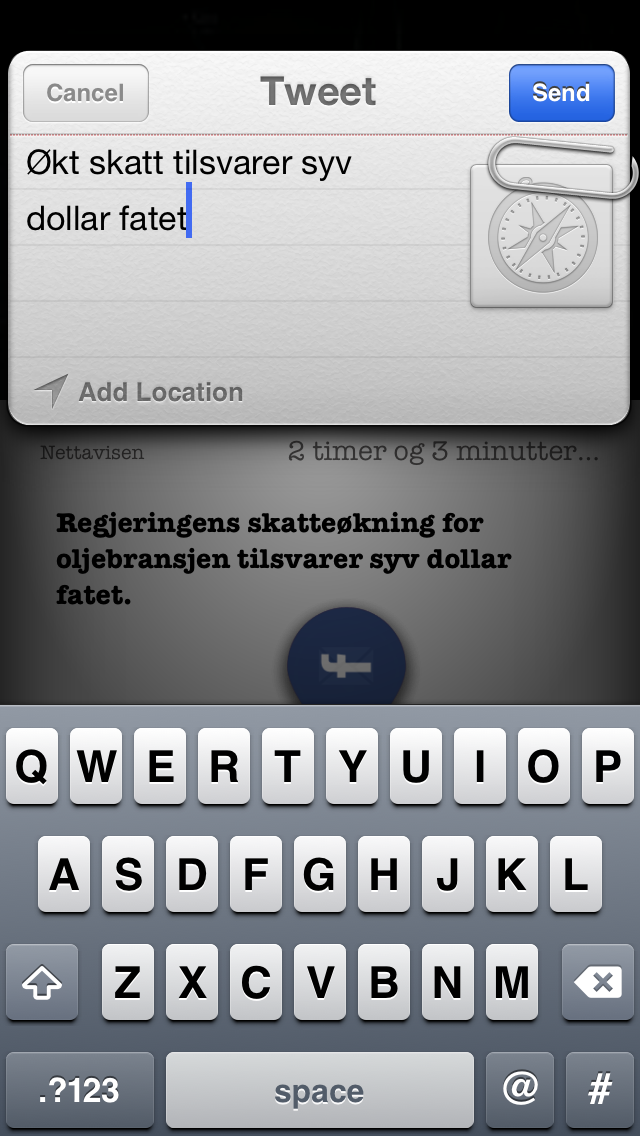
\includegraphics[width=49mm]{GFX/usecase/twitter.png}
\caption{Screenshot of the use case application showing the Twitter share screen.}
\label{usecase_twitter}
\end{figure}

\begin{figure}[!htbp]
\centering
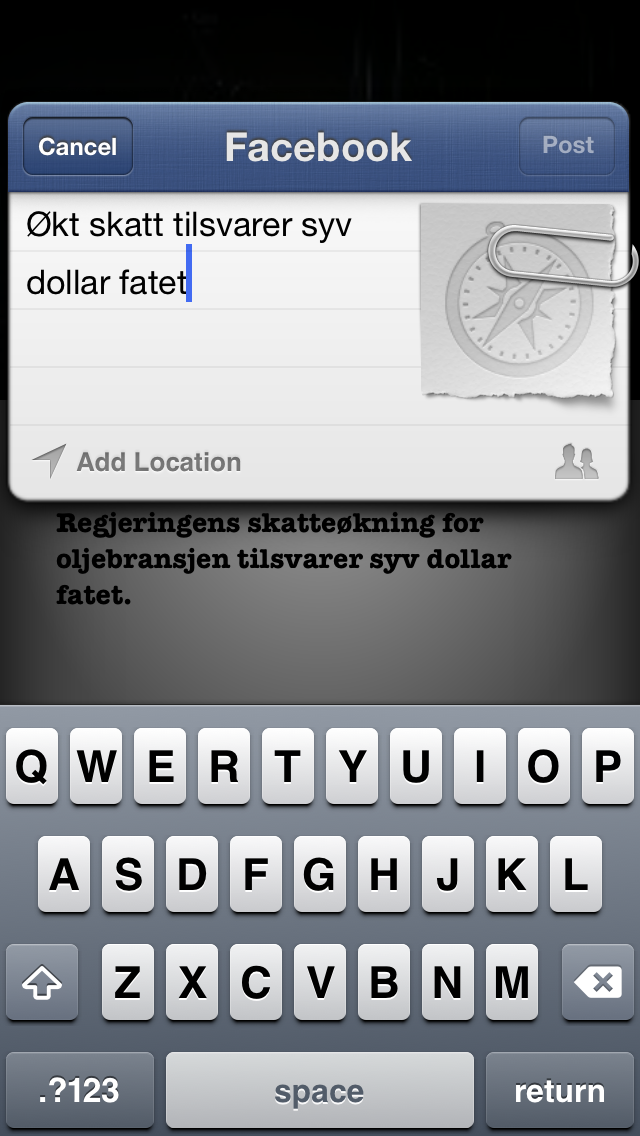
\includegraphics[width=49mm]{GFX/usecase/facebook.png}
\caption{Screenshot of the use case application showing the Facebook share screen.}
\label{usecase_facebook}
\end{figure}

\begin{figure}[!htbp]
\centering
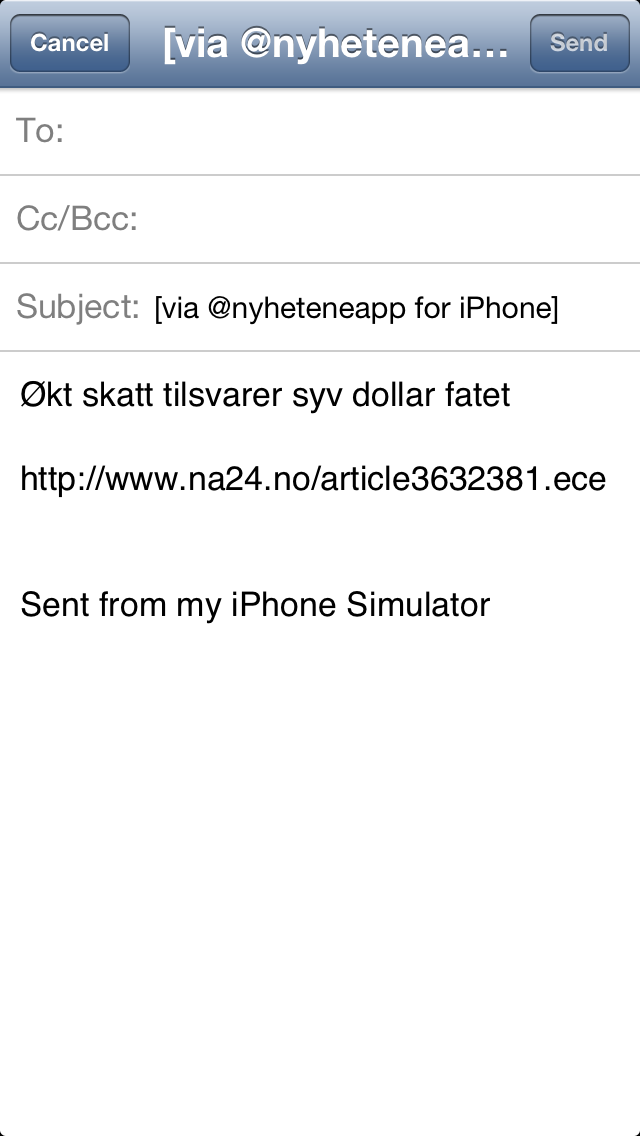
\includegraphics[width=49mm]{GFX/usecase/mail.png}
\caption{Screenshot of the use case application showing the email share screen.}
\label{usecase_mail}
\end{figure}

\begin{figure}[!htbp]
\centering
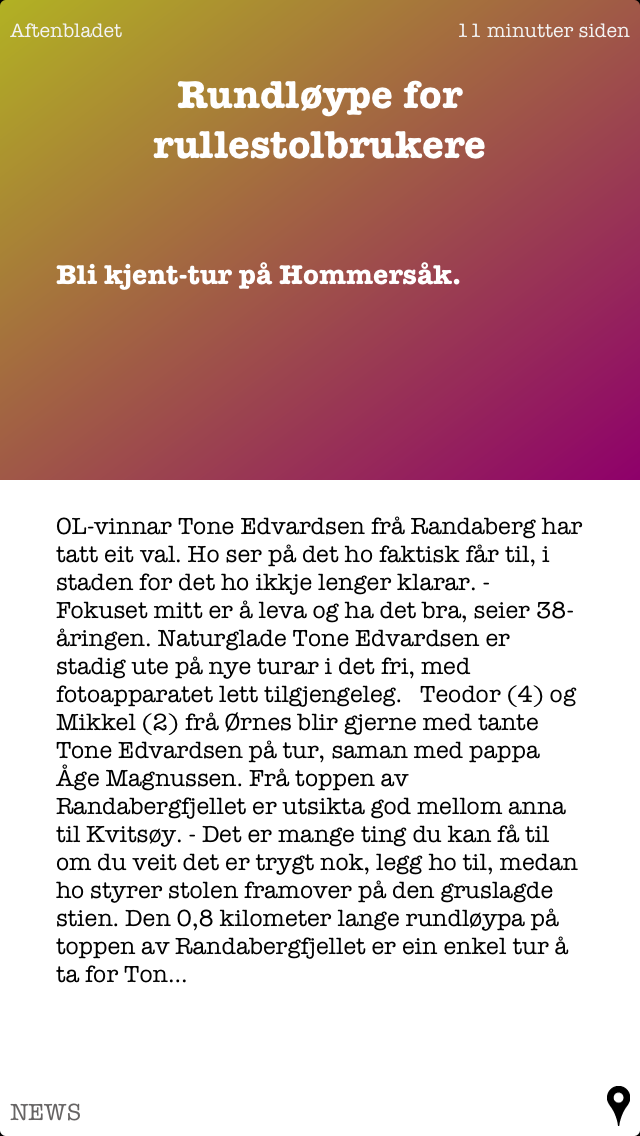
\includegraphics[width=49mm]{GFX/usecase/article.png}
\caption{Screenshot of the use case application showing the full article perspective.}
\label{usecase_article}
\end{figure}

\begin{figure}[!htbp]
\centering
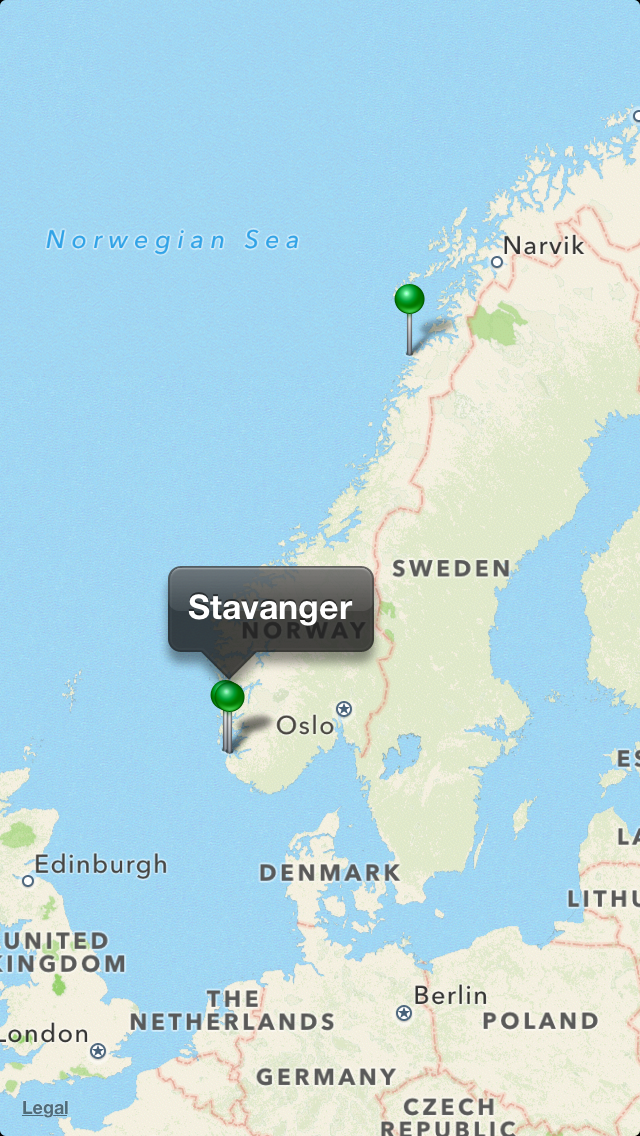
\includegraphics[width=49mm]{GFX/usecase/map.png}
\caption{Screenshot of the use case application showing the map perspective.}
\label{usecase_map}
\end{figure}

\begin{figure}[!htbp]
\centering
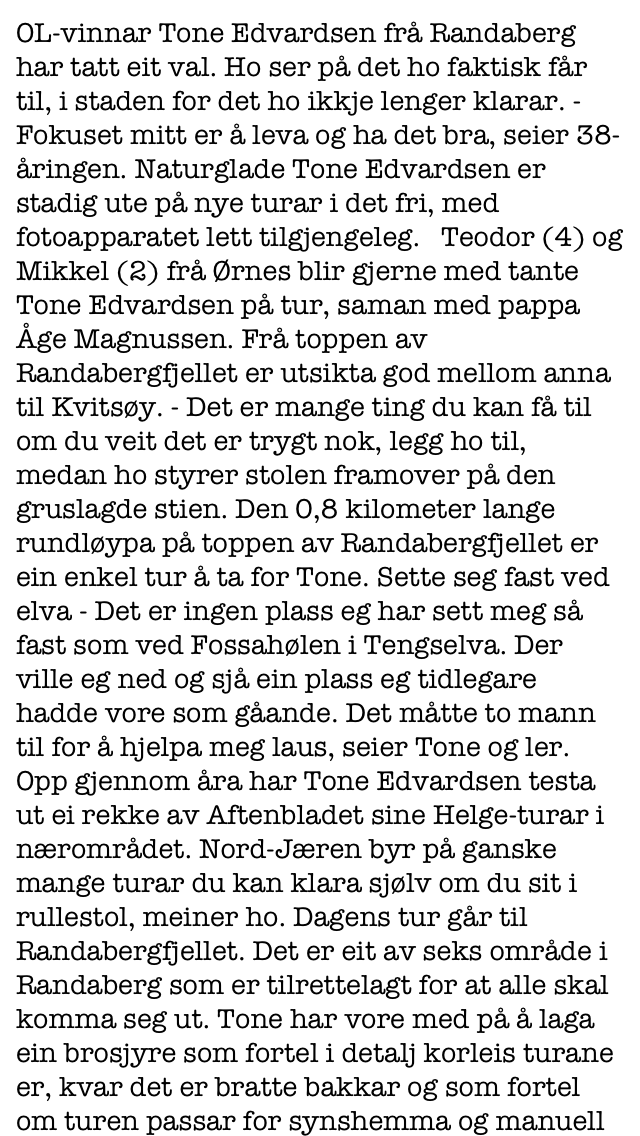
\includegraphics[width=49mm]{GFX/usecase/text.png}
\caption{Screenshot of the use case application showing the full text screen.}
\label{usecase_text}
\end{figure}

